\documentclass[a4paper,14pt,onecolumn]{article}


\usepackage[dvips]{graphics}
\usepackage{color}
\usepackage{epsfig}
\usepackage{amsmath}
\usepackage{graphicx}
\bibliographystyle{ieeetr}

\setlength{\textwidth}{6.27in}
\setlength{\textheight}{9.69in}
\setlength{\topmargin}{0.0in}
\setlength{\oddsidemargin}{0.0in}			% Customisable
\setlength{\headheight}{0.0in}
\setlength{\headsep}{0.0in}
\setlength{\topskip}{0.0in}

\fontencoding{T1}		% Font specification : Times New Roman, Bold, Normal, 18
\fontfamily{cmr}		% Roman
\fontseries{m}			% Medium
\fontshape{n}			% Upright
\fontsize{14pt}{5}		
\linespread{1.5}		% Vertical spacing between lines
\selectfont			% Select the specified font

\begin{document}
\pagestyle{empty}
%_____________________________________________________________________________________________ 
% Title page: Specifies a custom-made title page
%_____________________________________________________________________________________________ 
\DeclareGraphicsExtensions{.png, .ps}
\begin{titlepage}
\begin{center}
\Large{\bf{A PROJECT REPORT\\}}		% Large = 14.40
\Large{\bf{ON\\}}		% Large = 14.40
\begin{center}\color{blue}
\LARGE{\bf{ ``MINING CLASSIFICATION RULES FROM DATABASE USING ARTIFICIAL NEURAL NETWORK''\\}}	% LARGE = 17.28
\end{center}
\Large{Under the guidance of\\ }\begin{center}\color{red}
\Large{\bf{HOD Prof. Mrs. S. Shinde}\\}\end{center}
\vspace{8pt}
\Large{\em{Submitted by\\}}
\begin{table}[htbp]
	\begin{center}
    \color{red}
	\begin{tabular}{ l c c l }
	\Large{B8338503} & & & \Large{Prashant  P. Avaghade} \\ 
	\Large{B8338513} & & & \Large{Datta G. Diware} \\
	\Large{B8338528} & & & \Large{Mahesh S. kshatriya} \\
	\Large{B8338559} & & & \Large{Nikhilesh S. Shinde} \\
      \Large{B8338570} & & & \Large{Sumit S.Wankhede} \\
	\end{tabular}
	\end{center}
	\end{table}
%names of advisors
\Large{\em{Towards the Partial fulfillment of
Final year degree course in\\B.E. Information Technology\\
Of\\University of Pune
In the academic year
2011-12
\\}}
\vspace{3pt}
\vspace{10pt}
%pccoe logo added
\begin{figure}[h]
\centering

\includegraphics[width=3cm,height=3cm]{pccoelogo.jpg}
\end{figure}
\Large{\bf{DEPARTMENT OF INFORMATION TECHNOLOGY,\\ 
PIMPRI CHINCHWAD COLLEGE OF ENGINEERING, PUNE-46}}
\vfill
\large\bf{(2011-2012)}
\end{center}
\end{titlepage}

\thispagestyle{empty}
\begin{titlepage}
\begin{center}
\Large{\bf{PIMPRI CHINCHWAD EDUCATION TRUST’S
PIMPRI CHINCHWADCOLLEGE OF ENGINEERING
AKURDI, PUNE-411044
\\}}
\end{center}
\begin{center}
\color{red}\Huge{\bf{CERTIFICATE\\}}	
\end{center}
\begin{center}
\bf{
This is to certify that\\
Project work\\
ON}
\end{center}
\begin{center}
\color{blue}\LARGE{\bf{``MINING CLASSIFICATION RULES FROM DATABASE USING ARTIFICIAL NEURAL NETWORK'' \\}}	
\end{center}
\begin{center}
\Large{\em{Submitted by\\}}
\begin{table}[htbp]\color{red}
	\begin{center}
	\begin{tabular}{ l c c l }
	\Large{B8338503} & & & \Large{Prashant  P. Avaghade} \\ 
	\Large{B8338513} & & & \Large{Datta G. Diware} \\
	\Large{B8338528} & & & \Large{Mahesh S. kshatriya} \\
	\Large{B8338559} & & & \Large{Nikhilesh S. Shinde} \\
      \Large{B8338570} & & & \Large{Sumit S.Wankhede} \\
	\end{tabular}
	\end{center}
	\end{table}
%names of advisors


\Large{Under the guidance of\\ }\begin{center}
\color{red}\Large{\bf{HOD Prof. Mrs. S. Shinde}\\}\end{center}
\Large{Towards the Partial fulfillment of
Final year degree course in\\B.E. Information Technology
Of\\University of Pune
In the academic year
2011-12
\\}
\vspace{3pt}

% Horizontal spacing used to keep the signatures in columns at the ends of lines

%SIGNATURE\hspace{\stretch{1}}SIGNATURE\\
	\begin{table}[htbp]
	\begin{center}
	\begin{tabular}{ l c c c c l }
	\bf{Prof. S. V. Shinde} & \bf{Prof. R. G. Pise} & \bf{Prof. S. V.Shinde} & \bf{Prof.A.M.Fulambarkar}\\[0.3cm] 
	\bf{Project Guide} & \bf{Project Coordinator} & \bf{HoD} & \bf{Principal}\\
	\end{tabular}
	\end{center}
	\end{table} 
\end{center}
\end{titlepage}
\newpage
\begin{titlepage}
\begin{center}
\huge{\bf{ABSTRACT\\}}\end{center}
\large{
The important task in data mining is the classification of the data into the predefined groups or classes. One of the commonly used classifier technique is Artificial Neural Networks (ANN) [1]. Although ANN usually reaches high classification accuracy, the obtained results sometimes may be incomprehensible [2]. Due to this fact various methods have been proposed to extract the rules from ANN which justifies the classification results given by ANN. For this the trained neural network is pruned for removing the inputs that are not needed for solving the problem. The pruned network serves to filter noise that might be present in the data [2]. The proposed research work shall be based on extracting optimized the rules from ANN which justifies the classification results given by ANN.}
\end{titlepage}

\pagenumbering{roman}		% Lowercase roman numbering for prelim sections


\newpage
\thispagestyle{empty}
\tableofcontents		% *Generate* the table of contents. No content - no table
				% LATEX needs to run 2-3 times over source to get this correct

\newpage
\listoftables


\newpage
\listoffigures

\newpage
\pagenumbering{arabic} % Change to Arabic numbers for main chapters.
\section{INTRODUCTION}
\subsection{Need}

          Neural Networks are successful in acquiring hidden knowledge in datasets. Their biggest weakness is that the knowledge they acquire is represented in a form not understandable to humans. Researchers tried to address this problem by extracting rules from trained Neural Networks. Most of the proposed rule extraction methods required specialized type of Neural Networks; some required binary inputs and some were computationally Lack of explanation capability is one of the most important reasons why Neural Networks do not get the necessary interest in some parts of the industry.\\
          In most of the real world applications (especially in safety critical applications) users want to know the reasoning behind the conclusion of a learning system or an expert system. Extracting If-Then rules is usually accepted as the best way of extracting the knowledge represented in the Neural Network. Rules extracted from the trained net can be used for explaining the reasoning behind the output of the system. They can also be used in other systems, like expert systems or in systems for discovering previously unknown features in the data (data mining).\\ 
          Generalization of the system can also be improved by having a better feature representation. Quality of the rules can be measured by Accuracy, Fidelity, and Comprehensibility. Fidelity is the fraction of instances on which Neural Network and the extracted rules give the same output. Comprehensibility is measured by the size of the rule set and by the number of antecedents in each rule.

\section{Basic Concepts}

\subsection{Data Mining}
                       Data mining (DM), also known as ‘‘knowledge discovery in databases” (KDD), is the process of discovering meaningful patterns in huge databases [3]. In addition, it is also an application that can provide significant competitive advantages for making the right decision.  DM is an explorative and complicated process involving multiple iterative steps.

\subsection{ Data Mining Tasks}
  \begin{itemize}
\item Classification              : Classifies a data item into one of several predefined categories.

\item Regression                 : Maps a data item to a real-valued prediction variable.

\item Clustering                  : Maps a data item into a cluster, where clusters are natural groupings of data items based on similarity metrics.

\item Association rules        : Describes association relationship among different attributes.

\item Summarization           : Provides a compact description for a subset of data.

\item Dependency modeling : Describes significant dependencies among variables.

\item Sequence analysis       : Models sequential patterns, like time-series analysis. The goal  is to model the state of the process generating the sequence or to extract and  report deviations and trends over time.
\end{itemize}

 \subsection{ Data Mining Classification}

  \subsubsection{ Classification Techniques}
 \begin{itemize}
\item Decision Tree based Methods
\item Rule-based Methods
\item Memory based reasoning
\item Genetic Algorithms
\item Support Vector Machines
\item Neural Networks 
\end{itemize}

\subsubsection{ Classification }
Learn a method for predicting the instance class from pre-labeled (classified) t  Instances.

\begin{figure}[hbp]
\begin{center}
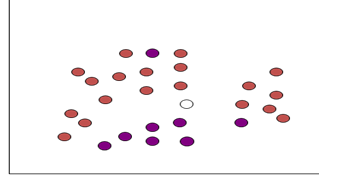
\includegraphics[height=3in,width=3in]
{classficationGraph.jpg}  
\caption{Classification Graph}
\end{center}
\end{figure} 

\subsubsection{  Decision Trees  }
            An internal node is a test on an attribute. A branch represents an outcome of the test, e.g. Color=red. A leaf node represents a class label or class label distribution. At each node, one attribute is chosen to split training examples into distinct classes as much as possible A new instance is classified by following a matching path to a leaf node.

\begin{figure}
\begin{center}
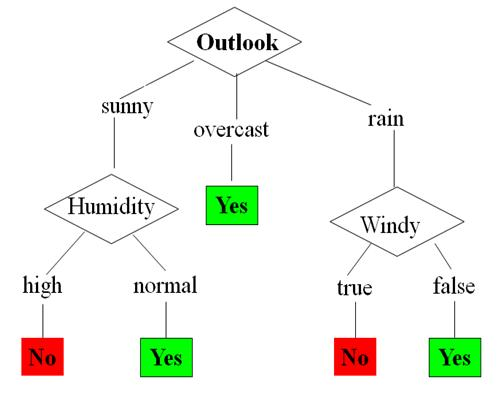
\includegraphics[height=4in,width=4in]
{decisiontree.jpg}  
\caption{Example Tree for “Play?”}
\end{center}
\end{figure} 

\subsection{Neural Network}

  \subsubsection{What is Neural Network?}
              A neural network is a powerful data modeling tool that is able to capture and represent complex input/output relationships. It is a biologically motivated approach to machine learning.


Neural networks resemble the human brain in the following two ways: 
 \begin{itemize}	
\item A neural network acquires knowledge through learning. 
\item A neural network's knowledge is stored within inter-neuron connection strengths known as synaptic weights.
\end{itemize}

\begin{figure}[hbp]
\begin{center}
\includegraphics[height=4in,width=4in]
{Neuron.jpg}  
\caption{Biological Neuron}
\end{center}
\end{figure}  

\begin{figure}[hbp]
\begin{center}
\includegraphics[height=4in,width=4in]
{Neuralnetwork.jpg}  
\caption{Basic Architecture of Neural Network}
\end{center}
\end{figure} 

  \subsubsection{Back propagation and Feed-Forward NN}
         It is a supervised learning method, and is a generalization of the delta rule. It requires a teacher that knows, or can calculate, the desired output for any input in the training set. It is most useful for feed-forward networks (networks that have no feedback, or simply, that have no connections that loop). The term is an abbreviation for "backward propagation of errors". Back propagation requires that the activation function used by the artificial neurons (or "nodes") be differentiable

\begin{figure}[hbp]
\begin{center}
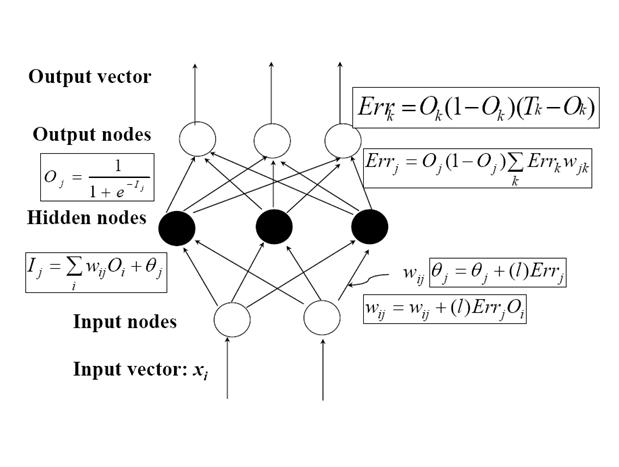
\includegraphics[height=4in,width=4in]
{BBNeuralnetwork.jpg}  
\caption{Backproagation Neural Network}
\end{center}
\end{figure} 

The ANN is composed of richly interconnected non-linear nodes that do processing in parallel. The connection weights are modifiable, allowing ANN to learn directly from examples without requiring or providing an analytical solution to the problem. The most popular forms of learning are:

\begin{itemize}

\item Supervised learning: Patterns for which both their inputs and outputs are known are presented to the ANN. The task of the supervised learner is to predict the value of the function for any valid input object after having seen a number of training examples. ANN employing supervised learning has been widely utilized for the solution of function approximation and classification problems.  

\item Unsupervised learning: Patterns are presented to the ANN in the form of feature values. It is distinguished from supervised learning by the fact that there is no a priori output. ANN employing unsupervised learning has been successfully employed for data mining and classification tasks. The self-organizing map (SOM) and adaptive resonance theory (ART) constitutes the most popular examples of this class. A backpropagation network (BPN) is a neural network that uses a supervised learning method and feed-forward architecture. A BPN is one of the most frequently utilized neural network techniques for classification and prediction and is considered an advanced multiple regression analysis that can accommodate complex and non-linear data relationships.
\end{itemize}

\subsubsection{Neural Network and data mining}
\begin{itemize}
\item Can select more complex regions.
\item Can be more accurate.
\item Also can overfit the data – find patterns in random noise.
\end{itemize}
\begin{figure}
\begin{center}
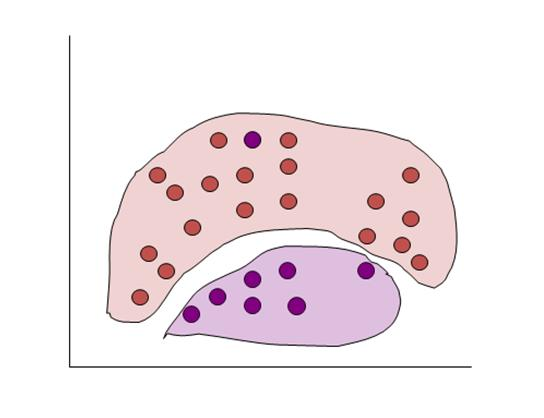
\includegraphics[height=3in,width=4in]
{NNdatamining.jpg}  
\caption{Neural Network in Data Mining}
\end{center}
\end{figure}

\subsubsection{Application}

\begin{itemize}
\item Key finance decision making problem e.g. credit card approval.
\item Medical Application e.g. cancer patient classification depending upon symptoms attributes.
\item Pattern Recognition.
\item Image Processing.
\end{itemize}

\newpage
\section{Literature Survey}
          To reveal the information concealed in an ANN, researchers have proposed a number of rule extraction techniques. One of the first rule extraction techniques from neural network was proposed by Galant . He was working on connectionist expert systems. In this work, each ANN node is represented as a conceptual entity.\\
     Yueh-Min Huanga and  Chun-Min Hunga [8] have  addressed the problem of imbalanced class distributions. This paper analyzes different classification algorithms that were employed to predict the creditworthiness of a bank’s customers based on checking account information. A series of experiments were conducted to test the different techniques. The objective is to determine a range of credit scores that could be implemented by a manager for risk management. Also a strategy of data cleaning for handling such a real case with imbalanced distribution data is presented by them.\\
      Wei-Sen Chen  and Yin-Kuan Du  have used the artificial neural network (ANN) and data mining (DM) techniques to construct the financial distress prediction model . In this paper traditional Data Mining- Clustering approach is compared with ANN approach. After this experimentation authors have stated that the ANN approach obtains better prediction accuracy than the DM clustering approach. Therefore, the authors have concluded that the artificial intelligent (AI) approach could be a more suitable methodology than traditional statistics for predicting the potential financial distress of a company.\\
      Humar Kahramanli and  Novruz Allahverdi [7] have presented the technique of mining the classification rules for Liver Disorders using adaptive activation function. In this study the authors have first trained the neural network with adaptive activation function. Then the rules are extracted from this trained neural network by using the OptaiNET that is an Artificial Immune Algorithm (AIS).\\
    The used Neuro-Adaptive function is as follows:\\

$Ø(x) ={A1e^{- x2}+A2}/{(1+e^{-B*x})}$\\
\\
Where, A1, A2 and B are real variables which will be adjusted during training.
     In this paper, for rule extraction the first ANN which classifies the dataset was designed. Then Opt-aiNET algorithm was executed for extraction of rules from this ANN. Finally, the extracted rules were decoded. Produced rules diagnosed correctly 192 samples from 200 belong to Class 0 and 135 samples from 145 belongs to Class1. It means system achieve 96% and 93% correctly diagnosis for Class 0 and Class 1 respectively. In summary the system correctly diagnosed 94.8% of whole samples.\\
     In paper [9] association rules have been composed using Apriori algorithm and transactions, which provide these rules, were eliminated. This provides shrinking database. Then ANN has been trained and used Opt-aiNET for composing rule set. It’s been observed that this method increased classification accuracy despite decreasing number of rules.\\ 
     Humar Kahramanli and  Novruz Allahverdi [1] have presented the method that uses Artificial Immune Systems (AIS) algorithm to extract rules from trained hybrid neural network [6]. The datasets used are Cleveland heart disease and Hepatitis data taken from UCI machine learning repository.\\ 
     The performance metrics used in this algorithm are accuracy, sensitivity and specificity which are the common performance metrics used in medical diagnosis tasks. The measure of the ability of the classifier to produce accurate diagnosis is determined by accuracy. The measure of the ability of the model to identify the occurrence of a target class accurately is determined by sensitivity. The measure of the ability of the model to separate the target class is determined by specificity. So that accuracy, sensitivity and specificity are calculated as follows:\\


$Accuracy=\frac{Total number of correctly diagnosed cases}{Total number of cases}$\\[4mm]

$Sensitivity=\frac{Total number of positive cases correctly diagnosed}{Total number of positive cases }$\\[4mm]

$Specificity=\frac{Total number of negative cases correctly diagnosedT}{Total number of negative cases}$\\[4mm]

     This method achieves accuracy values of 96.4% and 96.8% for Cleveland heart disease dataset and Hepatitis dataset respectively.\\
     Miguel Rocha and Paulo Cortez [10] have presented the use of Evolutionary Computation (EC) as a promising alternative for ANN optimization. In this paper two hybrid EC/ANN algorithms are presented: the first evolves neural topologies while the latter performs simultaneous optimization of architectures and weights. Sixteen real-world tasks were used to test these strategies. \\
      Richi Nayak [11] has given a novel methodology “Gyan” that represents the knowledge of a trained network in the form of restricted first-order predicate rules. \\
      In paper [5] the mathematical properties of several error functions with a focus on MLP data classification are analyzed. This analysis led us to propose two parameterized error functions for MLP training. The first one, ESMF, is a monotonic error function applicable only to two-class problems and was shown to perform equally well as other functions. However, it should be extended to the general multi-class problem for a better evaluation of its capability. The second one, EExp, an exponential-type error function, this function is able to emulate the behaviors of classic error functions and, as a matter of fact, by single parameter adjustment it is able to implement an infinite family of error functions, with different behavior of the error gradient weighting.\\
       By Ajit Narayanan, Edward Keedwell and Dragan Savic [12] have presented a novel approach using genetic algorithms to search for symbolic rules in a trained neural network.       Many rule extraction algorithms have been designed to generate classification rules from NNs that have been trained to distinguish data samples from different classes. These algorithms frequently assume that the input data attributes are discrete in order to make the rule extraction process more manageable. NeuroRule [14] is one such algorithm. A component of NeuroRule is an automatic rule generation method called rule generation (RG). Each rule is generated by RG such that it covers as many samples from the same class as possible with the minimum number of attributes in the rule condition. RG is applied to generate rules that explain the network’s output in terms of the discretized hidden unit activation values and rules that explain the discretized activation values in terms of the discretized attributes of the input data.\\
       Rule eXtraction (RX) [15] is another NN rule extraction algorithm that works on discrete data. RX recursively generates rules by analyzing the discretized hidden unit activations of a pruned network with one hidden layer. When the number of input connections to a hidden unit is larger than a certain threshold, a new NN is created and trained with the discretized activation values as the target output. \\
     The generalized analytic rule extraction (GLARE) algorithm [16] does not require network pruning. It does, however, require that the continuous attributes be first converted to nominal, and then to binary attributes before the algorithm can be applied. While the algorithm is shown to work well on discrete data sets, it does not perform as well as decision tree methods on data sets with continuous attributes. \\
     The orthogonal search-based rule extraction (OSRE) method [17] assumes that the data has been 1-from-N encoded; hence its application is also limited to data with only nominal or ordinal attributes. \\
    Trepan, an algorithm that was developed by Craven and Shavlik [18] also extracts M-of-N rules from an NN. It treats the NN as an oracle to generate additional data samples. This is an important step in trepan as it grows a decision tree by recursive partitioning. As the tree grows, fewer and fewer training samples are available for deciding if a node should be split further. Additional samples are generated by taking into account the distribution of the existing data samples and their labels are determined by the NN oracle. A node in the tree becomes a leaf node if it has sufficiently a high proportion of samples that belong to one class or if the number of internal nodes in the tree has reached the maximum.\\
    There exist algorithms that generate fuzzy rules from NNs. Nefclass [19] is one such algorithm. It works as a three-layer fuzzy NN. The difference between this type of networks and the standard backpropagation NNs lies in the connection weights which represent fuzzy sets and in the activation functions which act as fuzzy set operators. Nefclass employs a fuzzy variant of the backpropagation algorithm to find the characteristic parameters of the membership functions.\\
    Benitez [20] proposed a method for translating the knowledge embedded in an NN into a fuzzy-rule-based system.\\
    Tsukimoto [21] developed an NN rule extraction algorithm that could be applied to continuous data directly. Instead of linear combinations of the inputs as the rule conditions, the rules are represented as continuous Boolean function of the attributes. The algorithm has been tested only on the Iris data set and the accuracy obtained was not as good as the accuracy of the decision tree method C4.5.\\
    The algorithm full rule extraction (full-RE) [22] is able to extract accurate rules from the Iris data set without the need to binarize or normalize the continuous attributes of the data prior to network training. For each hidden node in the network, full-RE generates an intermediate rule that predicts its output according to the linear combinations of the input attributes. In order to obtain the final set of classification rules that do not involve network weights in their rule conditions, full-RE discretizes the input attributes and then solves a linear programming problem to select the relevant discretization boundary.\\
    A recent rule extraction algorithm that works on discrete and continuous data was proposed by Rabuñal [23]. There is, however, no provision for generating rules with separate rule conditions involving discrete and continuous attributes.\\
     Rudy Setiono and Bart Baesens [2] have presented a recursive algorithm for extracting classification rules (RE-RX) from feedforward neural networks that have been trained on data sets having both discrete and continuous attributes. This algorithm shares some similarities with other existing rule extraction algorithms. It assumes that the trained network has been pruned so that irrelevant and redundant network connections and units have been removed. It also makes use of the decision tree method C4.5 to generate rules with only discrete attributes in their conditions. The novel feature of the proposed recursive algorithm lies in the rule set generated. The rules are hierarchical such that only those rules at the deepest level have rule conditions that involve linear combinations of the continuous attributes, while the conditions of all the other rules involve only the discrete attributes. We believe that such rule conditions would greatly increase the comprehensibility of the rules, and hence greatly pave the way to open the NN “black box” wider.\\

\newpage
\section{Project Overview}

 \subsection{Project Statement}
 Mining classification rules from database using ANN and optimizing the knowledge generated in terms of classification accuracy.\\

 \subsection{Proposing theme of the project}
Recursive Neural Network Rule Extraction for Data with Mixed attributes By Rudy Setiono,Senior Member, IEEE, Bart Baesens, and Christophe Mues [IEEE Transaction on Neural Networks, Vol. 19 No. 2, February 2008 pp. 299-307]
In this paper, a recursive algorithm for extracting classification rules from feedforward neural networks that have been trained on data sets having both discrete and continuous attributes is presented Real-world classification problems usually involve both discrete and continuous input attributes. For such problems, all the continuous attributes must be discretized if algorithms such as NeuroRule, GLARE, and OSRE are to be used for rule extraction.The drawback of discretizing the continuous attributes is that the accuracy of the networks, and hence the accuracy of the rules extracted from the networks, may decrease. This is because discretization leads to a division of the input space into hyperrectangular regions. Each condition of the extracted rulescorresponds to one of these hyperrectangular regions where all data samples are predicted to belong to one class. Clearly, a data preprocessing step that divides the input space into rectangular subregions may impose unnecessary restrictions on the NNs as classifiers. It is highly likely that the boundaries of the regions that contain data samples from the same class are nonrectangular given that some of the data attributes are continuous.\\

\subsection{Methodologies/Techniques to be used for knowledge extraction}
\begin{enumerate}
\item The Multilayer Perceptrons are used in this study make use of biases, sigmoid       activation functions and one hidden layer with a variable number of nodes.
\item Back propagation algorithm for training ANN (Gradient steepest descent algorithm)
\item C 4.5 algorithm
\item MATLAB (MATrix Laboratory) Neural Network Toolbox 4.0 from Math Works Corp. is applied to perform the training exercises. 
\item Neural network packages: Neurodimensions’ Neurosolutions v3.0 and Thinkspro v1.05 by Logical Designs Consulting.
\item Support  Vector Machine algorithm
\item Credit Approval dataset from UCI machine repository.
\item Pruning algorithm
\end{enumerate}

\newpage
\section{System requirement and specification}

\subsection{Process Flow}
\begin{figure}
\begin{center}
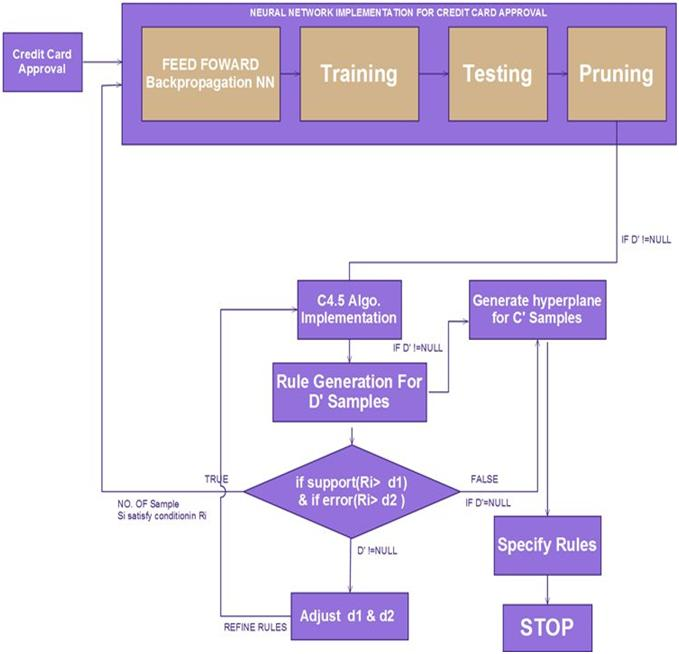
\includegraphics[scale=0.5mm]
{blockdiagram.jpg} 
\caption{Neural Network Implementation}
\end{center}
\end{figure}

\subsection{UML diagrams}

\susubsection{Use Case Diagram}
\begin{figure}
\begin{center}
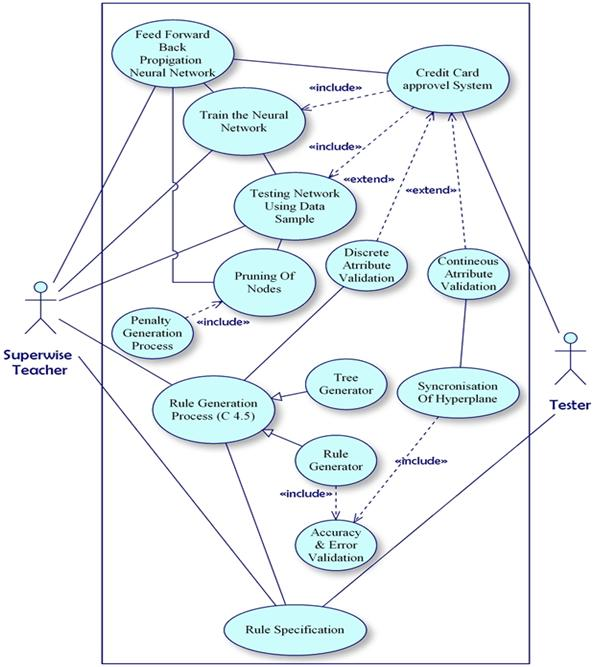
\includegraphics[scale=0.5mm]
{UseCaseForReport.jpg} 
\caption{Use cases}
\end{center}
\end{figure}
\end{document}
